\documentclass{beamer}

\usepackage{amsmath}
\usepackage{tikz}
\usepackage{fancyvrb}
\usepackage{textcomp}

\title{Transmembrane Protein Prediction using Long Short-Term Memory Networks}
\author{Kasper Lynderup Jensen}
\date{\today}

\begin{document}
\begin{frame}
\maketitle
\end{frame}

\begin{frame}<1>[label=tmp]
\frametitle<1>{Transmembrane proteins}
\frametitle<2>{Protein topology}
\centering
\includegraphics[width=\textwidth]{tmp.png}
\end{frame}

\begin{frame}[fragile, label=tmpp]
\frametitle{Transmembrane prediction}
\centering
\begin{BVerbatim}
...NTQYNSSYIFSITLVATLGGLLFGYDTAVISGTVESLNTVFVA...
...iiiiiiiiiiiiHHHHHHHHHHHHHHHHHHHHHoooooooooo...
\end{BVerbatim}
\end{frame}

\begin{frame}
\frametitle{Prediction methods}
\begin{columns}
	\begin{column}{0.5\textwidth}
		\begin{itemize}
			\item Hydrophobicity analysis
			\item Hidden Markov Models
			\item Artificial Neural Networks
		\end{itemize}
	\end{column}
	\begin{column}{0.5\textwidth}
		\begin{center}
			\includegraphics[width=\textwidth]{tmp.png}
		\end{center}
	\end{column}
\end{columns}
\end{frame}

\begin{frame}
\frametitle{TMSEG}
\centering
\includegraphics[width=\textwidth]{tmseg.jpg}
\end{frame}

\begin{frame}[fragile]
\frametitle{Prediction evaluation}
\centering
\begin{BVerbatim}
...NTQYNSSYIFSITLVATLGGLLFGYDTAVISGTVESLNTVFVA...
...iiiiiiiiiiiiHHHHHHHHHHHHHHHHHHHHHoooooooooo...
\end{BVerbatim}

\vspace{1cm}

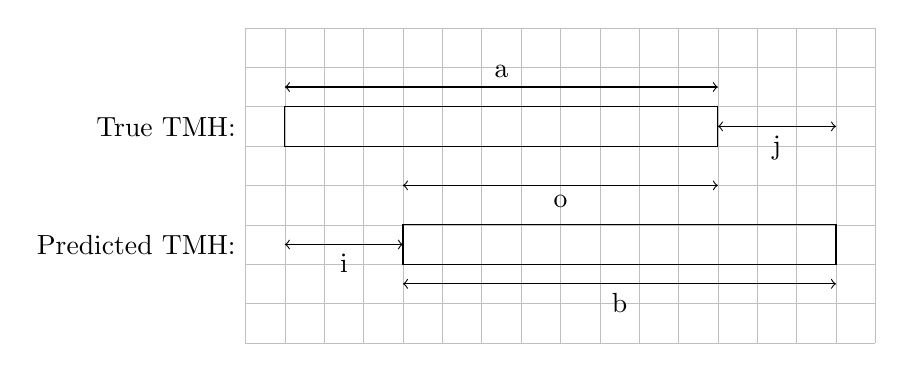
\begin{tikzpicture}[]
\draw[step=0.5cm,very thin,color=lightgray] (0,-1) grid (8,3);

\draw[] (0.5,1.5) rectangle (6,2);
\node at (-0,1.5) [anchor=south east] {True TMH:};
\draw[<->] (6,1.75) -- (7.5,1.75) node[pos=0.5, below]{j};
\draw[<->] (0.5,2.25) -- (6,2.25) node[pos=0.5, above]{a};

\draw[] (2,0) rectangle (7.5,0.5);
\node at (-0,0) [anchor=south east] {Predicted TMH:};
\draw[<->] (0.5,0.25) -- (2,0.25) node[pos=0.5, below]{i};
\draw[<->] (2,-0.25) -- (7.5,-0.25) node[pos=0.5, below]{b};

\draw[<->] (2,1) -- (6,1) node[pos=0.5, below]{o};
\end{tikzpicture}
\end{frame}

\begin{frame}
\frametitle{Artificial Neural Networks}
\centering
\includegraphics[width=\textwidth]{nn.jpg}
\end{frame}

\againframe{tmpp}

\begin{frame}
\frametitle{Recurrent Neural Networks}
\centering
\includegraphics[width=\textwidth]{RNN-unrolled.png}
\end{frame}

\begin{frame}
\frametitle{Long Short-Term Memory Networks}
\centering
\includegraphics[width=\textwidth]{LSTM3-chain.png}
\end{frame}

\begin{frame}[label=layout]
\frametitle{Model layout}
\centering
\resizebox{\textwidth}{!}{
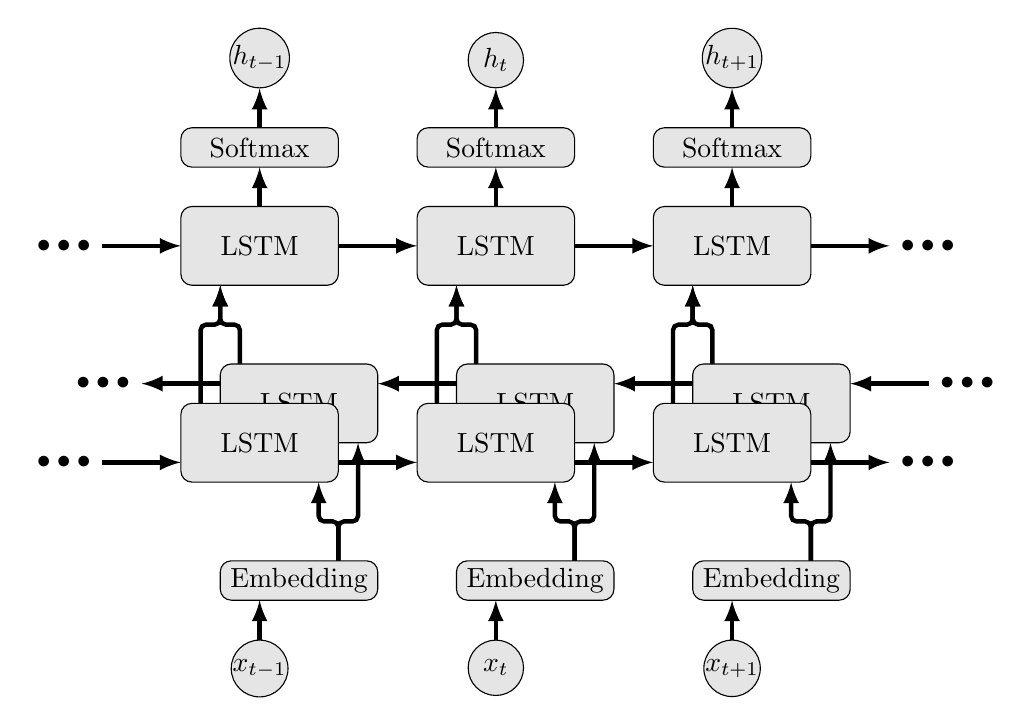
\begin{tikzpicture}[inputoutput/.style={circle, draw=black, fill=black!10, inner sep=0pt, minimum size=20pt, thin}]

% Output 
\draw[-latex, ultra thick] (-2, 4.5) -- (-2, 5) node[inputoutput, anchor=south] {$h_{t-1}$};
\draw[-latex, ultra thick] (1, 4.5) -- (1, 5) node[inputoutput, anchor=south] {$h_{t}$};
\draw[-latex, ultra thick] (4, 4.5) -- (4, 5) node[inputoutput, anchor=south] {$h_{t+1}$};

% Softmax	
\draw[rounded corners, fill=black!10] (-3, 4) rectangle (-1, 4.5) node[pos=.5] {Softmax};
\draw[rounded corners, fill=black!10] (0, 4) rectangle (2, 4.5) node[pos=.5] {Softmax};
\draw[rounded corners, fill=black!10] (3, 4) rectangle (5, 4.5) node[pos=.5] {Softmax};

\draw[-latex, ultra thick] (-2, 3.5) -- (-2, 4);
\draw[-latex, ultra thick] (1, 3.5) -- (1, 4);
\draw[-latex, ultra thick] (4, 3.5) -- (4, 4);

% Forward lstm
\draw[rounded corners, fill=black!10] (-3, 2.5) rectangle (-1, 3.5) node[pos=.5] {LSTM};
\draw[rounded corners, fill=black!10] (0, 2.5) rectangle (2, 3.5) node[pos=.5] {LSTM};
\draw[rounded corners, fill=black!10] (3, 2.5) rectangle (5, 3.5) node[pos=.5] {LSTM};

\draw[-latex, ultra thick] (-4, 3) -- (-3, 3) node[pos=0, left]{$\bullet\bullet\bullet$};
\draw[-latex, ultra thick] (-1, 3) -- (0, 3);
\draw[-latex, ultra thick] (2, 3) -- (3, 3);
\draw[-latex, ultra thick] (5, 3) -- (6, 3) node[right]{$\bullet\bullet\bullet$};

\draw[-latex, ultra thick, rounded corners=2pt] (-2.75, 1) |- (-2.5, 2) -- (-2.5, 2.5);
\draw[-latex, ultra thick, rounded corners=2pt] (-2.25, 1.5) |- (-2.5, 2) -- (-2.5, 2.5);

\draw[-latex, ultra thick, rounded corners=2pt] (0.25, 1) |- (0.5, 2) -- (0.5, 2.5);
\draw[-latex, ultra thick, rounded corners=2pt] (0.75, 1.5) |- (0.5, 2) -- (0.5, 2.5);

\draw[-latex, ultra thick, rounded corners=2pt] (3.25, 1) |- (3.5, 2) -- (3.5, 2.5);
\draw[-latex, ultra thick, rounded corners=2pt] (3.75, 1.5) |- (3.5, 2) -- (3.5, 2.5);

% Bidirectional lstm	
\draw[rounded corners, fill=black!10] (-2.5, 0.5) rectangle (-0.5, 1.5) node[pos=.5] {LSTM};
\draw[rounded corners, fill=black!10] (0.5, 0.5) rectangle (2.5, 1.5) node[pos=.5] {LSTM};
\draw[rounded corners, fill=black!10] (3.5, 0.5) rectangle (5.5, 1.5) node[pos=.5] {LSTM};

\draw[latex-, ultra thick] (-3.5, 1.25) -- (-2.5, 1.25) node[pos=0, left]{$\bullet\bullet\bullet$};
\draw[latex-, ultra thick] (-0.5, 1.25) -- (0.5, 1.25);
\draw[latex-, ultra thick] (2.5, 1.25) -- (3.5, 1.25);
\draw[latex-, ultra thick] (5.5, 1.25) -- (6.5, 1.25) node[right]{$\bullet\bullet\bullet$};

\draw[rounded corners, fill=black!10] (-3, 0) rectangle (-1, 1) node[pos=.5] {LSTM};
\draw[rounded corners, fill=black!10] (0, 0) rectangle (2, 1) node[pos=.5] {LSTM};
\draw[rounded corners, fill=black!10] (3, 0) rectangle (5, 1) node[pos=.5] {LSTM};

\draw[-latex, ultra thick] (-4, 0.25) -- (-3, 0.25) node[pos=0, left]{$\bullet\bullet\bullet$};
\draw[-latex, ultra thick] (-1, 0.25) -- (0, 0.25);
\draw[-latex, ultra thick] (2, 0.25) -- (3, 0.25);
\draw[-latex, ultra thick] (5, 0.25) -- (6, 0.25) node[right]{$\bullet\bullet\bullet$};

\draw[-latex, ultra thick, rounded corners=2pt] (-1,-1) -- (-1, -0.5) -| (-1.25, 0);
\draw[-latex, ultra thick, rounded corners=2pt] (-1,-1) -- (-1, -0.5) -| (-0.75, 0.5);

\draw[-latex, ultra thick, rounded corners=2pt] (2,-1) -- (2, -0.5) -| (1.75, 0);
\draw[-latex, ultra thick, rounded corners=2pt] (2,-1) -- (2, -0.5) -| (2.25, 0.5);

\draw[-latex, ultra thick, rounded corners=2pt] (5,-1) -- (5, -0.5) -| (4.75, 0);
\draw[-latex, ultra thick, rounded corners=2pt] (5,-1) -- (5, -0.5) -| (5.25, 0.5);

% embedding layer

\draw[rounded corners, fill=black!10] (-2.5, -1.5) rectangle (-0.5, -1) node[pos=.5] {Embedding};
\draw[rounded corners, fill=black!10] (0.5, -1.5) rectangle (2.5, -1) node[pos=.5] {Embedding};
\draw[rounded corners, fill=black!10] (3.5, -1.5) rectangle (5.5, -1) node[pos=.5] {Embedding};

% Input layer	
\draw[-latex, ultra thick] (-2, -2) -- (-2, -1.5) node[inputoutput, pos=0, anchor=north] {$x_{t-1}$};
\draw[-latex, ultra thick] (1, -2) -- (1, -1.5) node[inputoutput, pos=0, anchor=north] {$x_{t}$};
\draw[-latex, ultra thick] (4, -2) -- (4, -1.5) node[inputoutput, pos=0, anchor=north] {$x_{t+1}$};			
\end{tikzpicture}
}
\end{frame}

\begin{frame}
\frametitle{Results}
\centering 
\begin{tabular}{l|c|c} 
	Model & Precision & Recall \\ \hline
	Step 1 & $60 \pm 4$ & $61 \pm 5$ \\
	w PSSMs& $62 \pm 1$ & $65 \pm 2$ \\
	Step 2 & $65 \pm 5$ & $65 \pm 5$ \\
	w PSSMs& $67 \pm 3$ & $71 \pm 3$ \\
	Step 3 & $54 \pm 11$ & $54 \pm 13$ \\
	w PSSMs& $39 \pm 10$ & $40 \pm 9$ \\
	HMM   & $34 \pm 0$ & $13 \pm 0$ \\ 
	TMSEG & $87 \pm 3$ & $84 \pm 3$
\end{tabular}
\end{frame}

\begin{frame}
\frametitle{Run time}
\centering
\begin{tabular}{l|c|c} 
	Model & Training & Inference \\ \hline
	Step 1 & 800s & 1.61s \\ 
	Step 2 & - & 0.005s \\ 
	Step 3 & 1267s & 2.75s \\
	HMM   & 0.0495s & 0.80s
\end{tabular}

\begin{tabular}{rl}
Total inference time:& 4.37s for 41 proteins \\
My model per protein:& $\sim$100ms \\
TMSEG per protein:& $\sim$300ms
\end{tabular}
\end{frame}

\againframe<2>{tmp}

\begin{frame}
\frametitle{Hyper parameters}
\begin{columns}
	\begin{column}{0.5\textwidth}
		\begin{tabular}{l|c|c} 
			Model & Precision & Recall \\ \hline 
			Units=6 & $63 \pm 2$ & $64 \pm 2$ \\ 
			Units=10 & $65 \pm 3$ & $67 \pm 4$ \\ 
			Units=26 & $66 \pm 3$ & $68 \pm 4$ \\ 
			Units=50 & $66 \pm 3$ & $69 \pm 3$ \\ 
			Units=100 & $67 \pm 3$ & $69 \pm 4$ \\
		\end{tabular}
	\end{column}
	\begin{column}{0.5\textwidth}
		\begin{center}
			\includegraphics[width=\textwidth]{diff_units.png}
		\end{center}
	\end{column}
\end{columns}
\end{frame}

\end{document}